%==========================================================
% PART 3: rain maps and short forecasts (Phase 3).
%==========================================================
\clearpage
\begin{center}
\begin{minipage}{0.86\textwidth}
\small
\textbf{Part 3: from single links to rain maps and forecasts.} So far each link gave one number: the average rain along
its own beam. A flood warning needs more: rain \emph{everywhere} in a city, and a guess of where it will be in the next
hour. This part explains how we turn hundreds of link values into a map, how good those maps are when checked against
measurements the links never saw, and how far ahead the maps can be pushed. Same rules as before: every word explained,
real numbers only.
\end{minipage}
\end{center}

%==========================================================
\section{From lines to a map}
\label{sec:maps}
%==========================================================

A map is a grid of small squares, each with its own rain value. We have rain on lines (the links), and we need it on
squares. The simplest honest way is to let each square borrow from the links near it, trusting close links more than far
ones. This is called \textbf{inverse-distance weighting} (IDW).

\begin{enumerate}
\item Each link is represented by the point in the middle of its beam. (The two directions of one link are averaged
first: they share the same air.)
\item For a square, take its \textbf{8 nearest} links that are within \textbf{10\,km}.
\item Give each link a weight of $1/d^2$, where $d$ is its distance in kilometres. A link twice as far counts four times less.
\item The square's rain is the weighted average of those links' rain.
\item If no link is within 10\,km, the square gets \emph{no value}. We never invent rain where nothing measures it.
\end{enumerate}

\begin{example}[: one square, two links]
A square is 1\,km from link A, which reports 5\,mm/h, and 3\,km from link B, which reports 1\,mm/h. The weights are
$1/1^2 = 1$ and $1/3^2 = 0.11$. So
\[
R = \frac{1 \times 5 + 0.11 \times 1}{1 + 0.11} = \frac{5.11}{1.11} = 4.6\ \text{mm/h}.
\]
The square takes mostly after the close link A.
\end{example}

\begin{careful}
IDW cannot see rain between links: a shower that falls entirely between two dry links does not appear on the map.
And it smooths: the map is never wetter than the wettest nearby link. Cleverer methods exist (for example
\emph{kriging}, which learns from the data how fast rain changes with distance); IDW is our honest first step.
\end{careful}

%==========================================================
\section{How good are the maps?}
\label{sec:map_scores}
%==========================================================

A map is only worth something where it is checked against measurements that played no part in making it. We made hourly
maps from both methods (after the neighbour check, Section~\ref{sec:neighbours}) and checked them three ways.

\subsection{Sweden: the map at the rain gauges, against the radar}
In Gothenburg we read the map at the spot of each of the 10 city rain gauges (each 0.3--1.1\,km from the nearest link)
and compared it with what the gauge measured, hour by hour, through August 2015. As a yardstick, we did the same with the
weather radar.
\begin{center}\small
\begin{tabular}{lccccc}
\toprule
At the 10 gauges, hourly & $r$ & error (RMSE) & bias & CSI at 1\,mm/h\\
\midrule
Link map, classical & \textbf{0.92} & \textbf{0.72\,mm/h} & $-12\%$ & \textbf{0.74}\\
Link map, AI & 0.89 & 0.87\,mm/h & $-25\%$ & 0.67\\
Weather radar & 0.80 & 1.14\,mm/h & $\mathbf{+3\%}$ & 0.70\\
\bottomrule
\end{tabular}
\end{center}
(\textbf{CSI}, the critical success index, is explained in Section~\ref{sec:nowcast}: the share of ``rain above 1\,mm/h'' that
was in the right place, 1 being perfect.)

Where links are dense, \textbf{a map made from phone links follows the gauges better than the weather radar does}. It
measures a bit too little in total (the radar is almost exactly right in total), and, as in Part~2, the classical method
measures the Swedish amounts better than the AI.

\subsection{Italy: the map at rain gauges, near and far from links}
In Emilia-Romagna there are 319 weather stations with rain gauges, spread over the whole region, most of them nowhere
near a link. That lets us ask: how quickly does the map get worse as you move away from the links? We read the map at
every gauge and grouped the gauges by their distance to the nearest link.
\begin{center}\small
\begin{tabular}{lcccc}
\toprule
& \multicolumn{2}{c}{2021: $r$ / bias} & \multicolumn{2}{c}{2022: $r$ / bias}\\
\cmidrule(lr){2-3}\cmidrule(lr){4-5}
Gauge distance to nearest link & classical & AI & classical & AI\\
\midrule
0--2\,km (25 gauges) & 0.47 / $+54\%$ & \textbf{0.78 / $-13\%$} & 0.08 / $+190\%$ & \textbf{0.68 / $-19\%$}\\
2--5\,km (about 60) & 0.28 / $+73\%$ & \textbf{0.74 / $-13\%$} & 0.40 / $+43\%$ & \textbf{0.71 / $-15\%$}\\
5--10\,km (about 90) & 0.17 / $+67\%$ & \textbf{0.54 / $-20\%$} & 0.17 / $+38\%$ & \textbf{0.48 / $-20\%$}\\
\bottomrule
\end{tabular}
\end{center}
With the AI, the map is good within about 5\,km of a link ($r$ around 0.7--0.8) and clearly weaker beyond. The classical
maps inherit the classical method's trouble with Italy's 1-dB readings. And 145 of the 319 gauges are more than 10\,km
from any link, so they get no map at all: in a hilly region the phone network only covers where people live.

\subsection{The Netherlands: the whole map against the radar}
Here we compared the hourly map, square by square (2\,km squares, every square within 5\,km of a link: about 6{,}700 of
them), with KNMI's gauge-adjusted radar, through the summer of 2014.
\begin{center}\small
\begin{tabular}{lcccc}
\toprule
Every square, every hour & $r$ & error (RMSE) & bias & CSI at 1\,mm/h\\
\midrule
Link map, classical & 0.27 & 3.70\,mm/h & $+53\%$ & 0.44\\
Link map, AI & \textbf{0.59} & \textbf{1.57\,mm/h} & $\mathbf{+17\%}$ & \textbf{0.46}\\
\bottomrule
\end{tabular}
\end{center}

\begin{figure}[h]
\centering
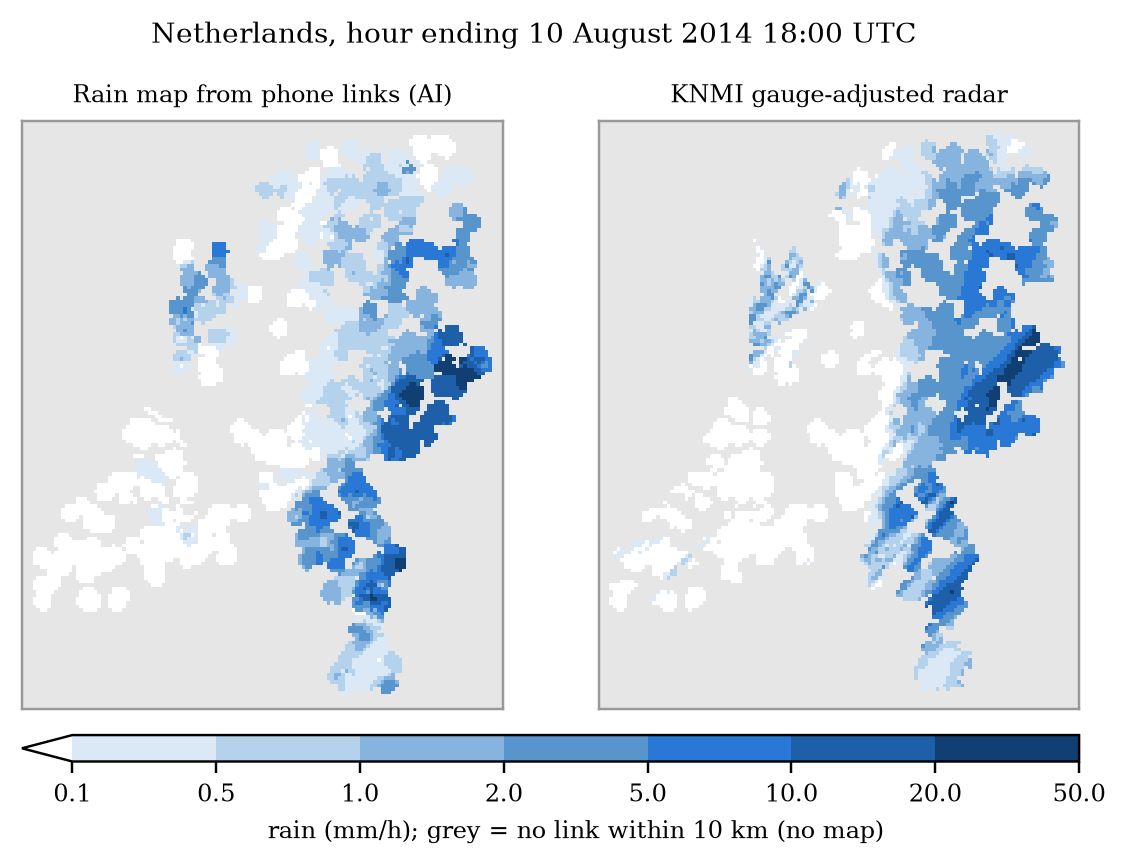
\includegraphics[width=0.82\textwidth]{fig_nl_map.png}
\caption{The wettest hour of the Dutch summer in our data. Left: rain map made only from phone links (AI, 1{,}653 sub-links).
Right: KNMI's gauge-adjusted radar for the same hour and the same squares. The link map gets the big picture right: the
band of rain from south to north-east, dry in the west, the heaviest cores in the east. It is blotchier (each link makes a
round patch around itself) and misses the finest detail.}
\label{fig:nl_map}
\end{figure}

\begin{oneline}
Where links are dense, a map made from them matches rain gauges better than a weather radar does; the map stays useful up to
about 5\,km from the nearest link and is blank beyond 10\,km.
\end{oneline}

%==========================================================
\section{Forecasting the next hour}
\label{sec:nowcast}
%==========================================================

A flood warning is most useful before the rain arrives. The simplest forecast of the next hour, called
\textbf{nowcasting}, does not need any weather physics: watch how the rain pattern moved over the last half hour and assume
it keeps moving the same way.

\subsection{How it works}
\begin{enumerate}
\item \textbf{Find the motion.} Take the last three maps (30 and 15 minutes ago, and now). For each part of the map, look
for the shift that best lines up the earlier pattern with the later one. This is called \textbf{optical flow}; it is the
same idea a phone camera uses to steady a shaky video. We used the Lucas--Kanade method from \textbf{pysteps}, a free
nowcasting toolkit used by weather services.
\item \textbf{Move the map.} Push every square of the current map along its arrow, 15 minutes at a time, up to 60 minutes
(\emph{semi-Lagrangian extrapolation}: each square of the forecast looks back along the arrows to find where its rain is
coming from).
\item \textbf{Compare with a lazy forecast.} \textbf{Persistence} assumes the rain stays exactly where it is now. A
nowcast is only worth something if it beats that.
\end{enumerate}

\subsection{Scoring a forecast: the critical success index}
Pick a threshold, say 1\,mm/h. Over all squares, count \textbf{hits} (forecast and observed both above it), \textbf{misses}
(observed above, forecast below) and \textbf{false alarms} (forecast above, observed below). Then
\[
\text{CSI} = \frac{\text{hits}}{\text{hits} + \text{misses} + \text{false alarms}} .
\]
1 is perfect; 0 means the forecast never put rain in the right place. Squares where both say ``dry'' do not count, so a
forecast cannot score well just by saying ``dry'' over a mostly dry country.

\begin{example}[: CSI]
On one map, 300 squares are forecast wet and 400 are observed wet; 200 of them overlap. Hits 200, misses
$400-200 = 200$, false alarms $300-200 = 100$. CSI $= 200 / (200+200+100) = 0.40$.
\end{example}

\subsection{Results}
We made a nowcast at every full hour of the Dutch summer when rain covered at least 800\,km$^2$ of the network: 612 hours.
\begin{center}
\begin{tikzpicture}
\begin{axis}[width=0.62\textwidth,height=5cm,xmin=10,xmax=65,ymin=0,ymax=0.5,xtick={15,30,45,60},
  xlabel={forecast lead time (minutes)},ylabel={CSI at 1 mm/h},grid=major,grid style={inkc!12},
  tick label style={font=\small},label style={font=\small},
  legend style={font=\scriptsize,draw=none,fill=white,fill opacity=0.85,text opacity=1},legend cell align=left,legend pos=north east]
  \addplot[thick,color=inkc,mark=*,mark size=1.6pt] table[x=lead,y=nowcast] {nowcast_csi.dat};
  \addlegendentry{nowcast (moving the map)}
  \addplot[thick,dashed,color=gaugec,mark=square*,mark size=1.4pt] table[x=lead,y=persistence] {nowcast_csi.dat};
  \addlegendentry{persistence (rain stays put)}
\end{axis}
\end{tikzpicture}
\end{center}
\begin{center}\small
\begin{tabular}{lcccc}
\toprule
Lead time & 15 min & 30 min & 45 min & 60 min\\
\midrule
CSI at 1\,mm/h, nowcast & \textbf{0.45} & \textbf{0.28} & \textbf{0.20} & \textbf{0.16}\\
CSI at 1\,mm/h, persistence & 0.44 & 0.27 & 0.19 & 0.15\\
\bottomrule
\end{tabular}
\end{center}
These scores compare the forecast with the link map that was actually observed later. As an independent check we also
compared the forecast rain for the whole next hour with KNMI's radar for that hour: CSI 0.26 for the nowcast against 0.24
for persistence, correlation 0.30 against 0.26.

\begin{figure}[h]
\centering
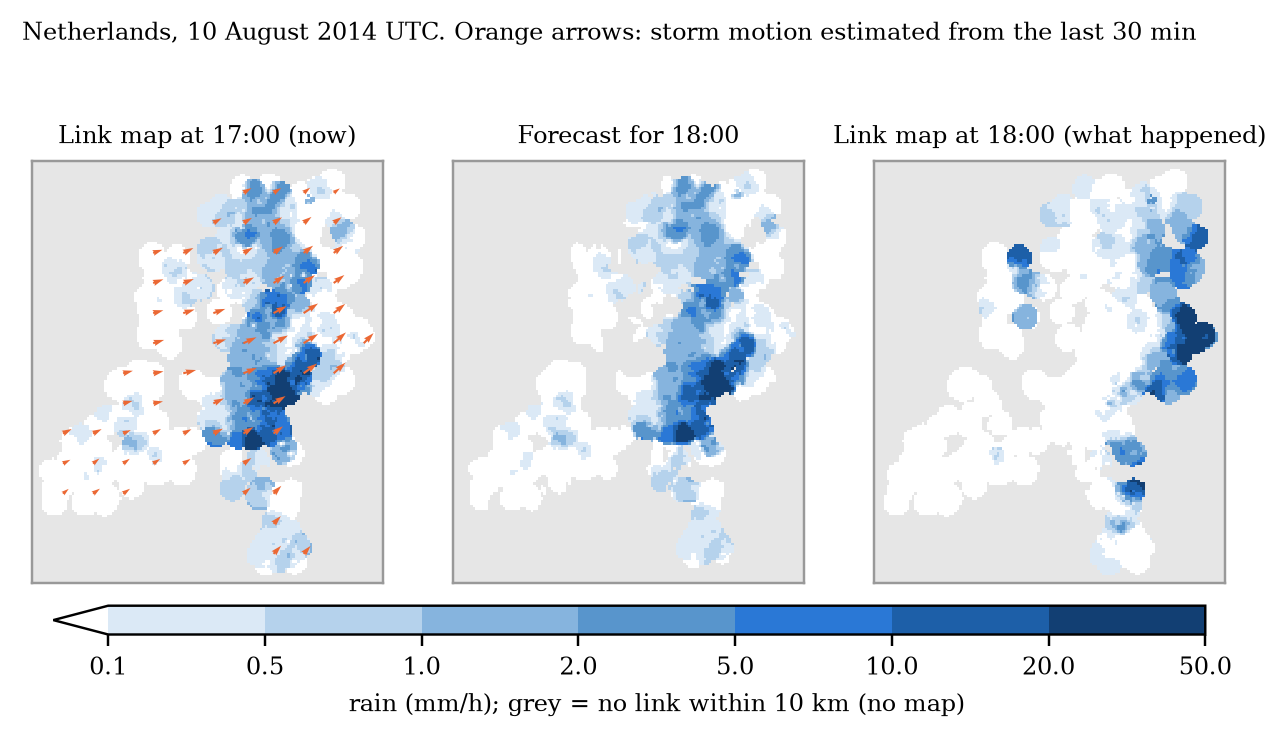
\includegraphics[width=0.95\textwidth]{fig_nowcast.png}
\caption{A nowcast during the same storm as Figure~\ref{fig:nl_map}. Left: the link map at 17:00 and the motion found from the
last 30 minutes (towards the north-east). Middle: that map moved forward 60 minutes. Right: what the links actually saw at
18:00. The direction was right, but the storm moved faster than forecast and by 18:00 its heaviest part was already
leaving the network on the east side.}
\label{fig:nowcast}
\end{figure}

\textbf{Honest reading.} The nowcast beats persistence at every lead time and in both checks, but only by a little. Skill
falls quickly: after 30 minutes, fewer than a third of the 1\,mm/h areas are in the right place. Three reasons, all visible
in Figure~\ref{fig:nowcast}:
\begin{itemize}
\item \textbf{Blotchy maps.} Each link makes a round patch on the map, and patches flicker as links switch between ``wet''
and ``dry''. Optical flow then partly tracks the flicker instead of the storm.
\item \textbf{Blind edges.} Rain that is about to enter the network from outside is invisible until it arrives, and rain
leaving it disappears. Radar sees 100+\,km beyond any city.
\item \textbf{Coarse steps.} The Dutch data come every 15 minutes; radar nowcasting usually uses 5-minute images.
\end{itemize}

\begin{oneline}
Moving the link map along the storm's motion gives a forecast that beats ``rain stays put'' up to an hour ahead, but only
slightly; for useful 30--60 minute warnings the motion should come from a wider view (radar or satellite), with the links
providing the accurate rain inside the city.
\end{oneline}

%==========================================================
\section{What Phase 3 taught us}
\label{sec:phase3_end}
%==========================================================

\begin{itemize}
\item \textbf{Maps from links work where links are.} In Gothenburg, link maps match rain gauges better than the weather
radar (correlation 0.92 and 0.89 against 0.80). In Italy and the Netherlands the AI maps are good within about 5\,km of a
link and far better than the classical ones.
\item \textbf{Coverage follows people.} Away from towns there are no links and no map: 145 of 319 Italian gauges are more
than 10\,km from any link. For Algeria this means link maps for cities and valleys with towers, and something else (radar
where it exists, satellites) everywhere else.
\item \textbf{Forecasting from links alone is weak.} The nowcast beats persistence, but by a small margin.
\end{itemize}

\textbf{Next:}
\begin{enumerate}
\item Better nowcasts by taking the storm motion from a wider view: satellite rain (NASA's IMERG, every 30 minutes,
worldwide), and radar where available, while keeping the links' accurate rain inside the city.
\item Phase~4: a simulated Algerian network on real tower positions, fed with real storms, to show the whole chain working
on Algeria (clearly labelled as a simulation).
\end{enumerate}
